\section{Differential cross-section}

The analysis method is very similar to the previously published ones \cite{prl111,epl101-el}. Each diagonal is analysed separately, some steps are performed independently for each bunch. In this analysis, however, a different normalisation approach is used, consequently making all $t$-independent scaling factors (e.g.~certain inefficiency corrections) irrelevant.

%----------------------------------------------------------------------------------------------------
\subsection{Event reconstruction}

Event kinematics is determined from track hits in RPs (after proper alignment, see Sec.~\ref{sec:alignment}) using the LHC optics (see Sec.~\ref{sec:optics}).

%------------------------------

\subsubsection{Kinematics determination}
\label{sec:kinematics}

The protons' kinematics is first reconstructed separately in each arm, using formulae that maximise the robustness against imperfections (predominantly optics):
%guide for reconstruction formulae = robustness against error sources: beam divergence, sensor pitch, misalignment, vertex term neglected, optics imperfections
\begin{equation}
\label{eq:kin 1a}
	\begin{aligned}
		\theta_x^* &= {v_x^{\rm N} x^{\rm F} - v_x^{\rm F} x^{\rm N}\over v_x^{\rm N} L_x^{\rm F} - v_x^{\rm F} L_x^{\rm N}}\ ,\qquad
		\theta_y^* = {1\over 2} \left( {y^{\rm N}\over L_y^{\rm N}} + {y^{\rm F}\over L_y^{\rm F}} \right)\ ,\\
		x^* &= {L_x^{\rm N} x^{\rm F} - L_x^{\rm F} x^{\rm N}\over L_x^{\rm N} v_x^{\rm F} - L_x^{\rm F} v_x^{\rm N}}\ , \\
	\end{aligned}
\end{equation}
where the N and F superscripts refer to the near and far units, $x$ and $y$ to horizontal and vertical track hits and $v$ and $L$ stand for the magnification and effective length optical functions. This reconstruction is used for tagging elastic events, where the left and right arm protons are compared. Once an event is selected, all four RPs can be used to reconstruct the kinematics of the event, in addition optimising for angular resolution:
\begin{equation}
\label{eq:kin 2a}
		\theta_x^* = {
				\sum {v_x^i}^2 \sum L_x^i x^i - \sum L_x^i v_x^i \sum v_x^i x^i
				\over
				\sum {v_x^i}^2 \sum {L_x^i}^2 - \sum L_x^i v_x^i \sum L_x^i v_x^i
			}\ ,\quad
		\theta_y^* = {1\over 4} \sum {y^i\over L_y^i}\ ,
\end{equation}
where the sums go over the superscripts $i$ representing the four RPs of a diagonal. Eventually, the full scattering angle, $\theta^*$, and four-momentum transfer squared, $t$, are calculated:

\begin{equation}
\label{eq:th t}
\theta^* = \sqrt{{\theta_x^*}^2 + {\theta_y^*}^2}\ ,\quad t = - p^2 ({\theta_x^*}^2 + {\theta_y^*}^2)\ ,
\end{equation}
where $p$ denotes the beam momentum.


%------------------------------

\subsubsection{Alignment}
\label{sec:alignment}

The standard three-step procedure \cite{totem-ijmp} has been applied: collimator-like alignment prior to run, track-based alignment (relative among RPs) and alignment with elastic events (absolute with respect to the beam). The procedure has been further extended by steps improving the vertical alignment. They exploit the fact that the elastic scattering with its two anti-collinear protons can relate the alignment in the left and right arm (with an uncertainty of $20\un{\mu m}$). Furthermore, the horizontal RPs in the right arm recorded a hit distribution usable for vertical alignment in addition to the standard technique based on the vertical RPs. Together, the two methods reduce the uncertainty to about $70\un{\mu m}$. The horizontal alignment and rotation about the beam have been determined by the standard approach, with uncertainties $30\un{\mu m}$ and $2\un{m rad}$, respectively. Propagating the uncertainties to the reconstructed angles, Eq.~(\ref{eq:kin 2a}), gives $0.28\un{\mu rad}$ ($0.19\un{\mu rad}$) for horizontal (vertical) angle. The error of the RP rotations would bias the reconstructed $\theta_x^*$ by a term proportional to $\theta_y^*$, with the proportionality constant having standard deviation $0.005$.

% the observed hit inefficiencies -- possible asymmetries -- discuss ???
% mention final alignment check = 2D Gaussian fit of $\theta_x^*$ vs.~$\theta_y^*$ from both diagonals ??

%------------------------------

\subsubsection{Optics}
\label{sec:optics}

In order to reduce errors due to imperfect optics knowledge, the optics matching technique \cite{totem-optics} has been applied. The residual uncertainty has a form of factors scaling the reconstructed scattering angles. For the double-arm reconstruction, Eq.~(\ref{eq:kin 2a}), the factors have standard deviations $0.34\un{\%}$ (horizontal) and $0.25\un{\%}$ (vertical), including the effects of magnet harmonics.


%------------------------------

\subsubsection{Resolution}
\label{sec:resolution}

Good knowledge of statistical fluctuations in the event reconstruction is essential for several steps in differential cross-section evaluation.

The fluctuations in $\theta_y^*$ are mostly due to the beam divergence and can be studied by comparing the angles reconstructed from the left and right arm. If the divergences of the two beams are the same (verified by emittance measurements with uncertainty of $25\un{\%}$), then the beam divergence distribution can be de-convoluted from the distribution of the left-right differences. The beam divergence has shown very small deviations from Gaussian shape but increasing width with time. Therefore, the $\theta_y^*$ (Eq.~(\ref{eq:kin 2a})) resolution degraded from initial $0.43$ to $0.48\un{\mu rad}$ at the end of the fill.

In the horizontal projection, a different method is used since the one-arm reconstruction, Eq.~(\ref{eq:kin 1a}), is strongly influenced by sensor resolution (strip pitch). First, the beam divergence is estimated from the vertex $x^*$ spread by dividing by $\beta^*$: it grew from $0.75$ to $0.9\un{\mu rad}$ during the fill. Then, the beam-divergence component is subtracted from the standard deviation of the right-left difference in $\theta_x^*$, yielding (time-independent) contribution from the sensor resolution: $10.7\un{\mu m}$ (45 top -- 56 bottom) and $12.1\un{\mu m}$ (45 bottom -- 56 top). This can be propagated to the two-arm resolution in $\theta_x^*$, Eq.~({\ref{eq:kin 2a}}), which is by far dominated the beam divergence component: it rose from $0.54$ to $0.65\un{\mu rad}$ during the fill. 


%----------------------------------------------------------------------------------------------------
\subsection{Differential cross-section reconstruction}
\label{sec:diff cs}

For a given $t$ bin, the value of differential cross-section is evaluated by selecting and counting elastic events as follows
\begin{equation}
{\d\sigma\over \d t}(\hbox{bin}) =
	{\cal N}\, {\cal U}({\rm bin})\, {\cal B}\ 
	{\sum\limits_{t \in \hbox{bin}} {\cal A}(\theta^*, \theta_y^*)\, {\cal E}(\theta_y^*)\over \Delta t}\ ,
\end{equation}
where $\Delta t$ is the width of the bin, ${\cal N}$ is a normalisation factor and the other symbols stand for various correction factors:
 ${\cal U}$ for unfolding of resolution effects, ${\cal B}$ for background subtraction, ${\cal A}$ for acceptance correction and ${\cal E}$ for detection and reconstruction efficiency.

%-------------------------

\subsubsection{Event tagging}
\label{sec:tagging}

The cuts used to select the elastic events are summarised in Table \ref{tab:cuts}, all are applied at $4\sigma$-level. Cuts 1 and 2 require the reconstructed-track collinearity between the left and right arm. Cut 3 ensures that the protons come from the same vertex (horizontally). Thanks to the very low beam divergence, the collinearity cuts are very stringent and consequently the other conceivable cuts (cf.~Table 2 in \cite{epl101-el}) bring no significant improvement.

The tagging efficiency has been studied by applying the cuts also at $5\un{\sigma}$-level. This selection has yielded $0.3\un{\%}$ more events, almost uniformly in $|t|$. This kind of inefficiency is irrelevant for the presented analysis.

\begin{table}
\caption{The elastic selection cuts. The superscripts R and L refer to the right and left arm. The $\alpha \theta_x^*$ term in cut 3 is intended to absorb possible effects of residual optics imperfections \todo{update at the end}. The right-most column gives a typical RMS of the cut distribution.
}
\label{tab:cuts}
\begin{center}
\vskip-3mm
\begin{tabular}{ccc}\hline\hline
number & cut & RMS ($\equiv 1\sigma$)\cr\hline
1 & $\theta_x^{*\rm R} - \theta_x^{*\rm L}$				& $3.9\un{\mu rad}$	\cr
2 & $\theta_y^{*\rm R} - \theta_y^{*\rm L}$				& $1.0\un{\mu rad}$	\cr
3 & $x^{*\rm R} - x^{*\rm L} - \alpha \theta_x^*$		& $250\un{\mu m}$ 	\cr\hline\hline
\end{tabular}
\end{center}
\end{table}


%-------------------------

\subsubsection{Background}
\label{sec:background}

To study the background (i.e.~impurity of the tagging), the distributions of right-left angular differences (see Table \ref{tab:cuts}) are plotted under various cut combinations. While the central part (signal) remains essentially constant, the tails (background) are dramatically affected. Interpolating the background smoothly to the signal region ($\pm 4\un{\sigma}$) permits to conclude negligible background: $1 - {\cal B} < 0.1\un{\%}$ (independently from $\theta_x^*$ and $\theta_y^*$ distributions). As an additional test, if a cut is released the recuperated events (less than $0.3\un{\%}$) are distributed almost uniformly over the $|t|$ range.

% background = impurity of the cuts above


%-------------------------

\subsubsection{Acceptance correction}
\label{sec:acc corr}

Beyond the usual acceptance limitations -- sensor edge (relevant for low $|\theta^*_y|$) and LHC apertures (high $|\theta_y^*|$) -- two additional ones have been identified. Both stem from the horizontal RPs interfering with the elastic protons, resulting in phase space region with uncertain detection efficiency. Consequently, an additional acceptance restriction $-50 < \theta_x^* < 80\un{\mu rad}$ has been adopted to avoid the interference regions. In far vertical RPs, the restriction corresponds to about $-2.3 < x < 3.7\un{mm}$.

The expected azimuthal symmetry of elastic scattering is verified for the data within acceptance. Assuming the symmetry globally yields a geometrical correction ${\cal A}_{\rm geom}(\theta^*)$ calculated from a fraction of circle with radius $\theta^*$ falling into the acceptance region in the $\theta_x^*$, $\theta_y^*$ space. The value of the correction drops rapidly from $10$ at the lowest $|t|$ to about $2$ at $|t| = 0.04\un{GeV^2}$ and then increases slowly to about $10$ as $|t|$ tends to $0.2\un{GeV^2}$.

The other acceptance correction, ${\cal A}_{\rm fluct}$, accounts for fluctuations around horizontal acceptance boundaries. It is calculated analytically from the probability that any of the two elastic protons is pushed outside the acceptance due to the beam divergence. The beam divergence distribution is modelled as Gaussian with spread determined in Section~\ref{sec:resolution}. This correction contribution is only relevant for low $|t|$ (below $0.002\un{GeV^2}$ for diagonal 45 top -- 56 bottom) and is limited below $2.5$. The uncertainties are related to the resolution parameters. For the lowest $|t|$ bin they yield: vertical beam divergence size $2\un{\%}$, left-right asymmetry $1\un{\%}$ and non-Gaussian shape $1\un{\%}$.

The final acceptance correction combines the two contributions:
\begin{equation}
{\cal A}(\theta^*, \theta_y^*) = {\cal A}_{\rm geom}(\theta^*)\ {\cal A}_{\rm fluct}(\theta_y^*)\ .
\end{equation}

\iffalse
\> A_g
\>> at low |t|: correction < 10 (for 1 diagonal)
\>> at high |t|: correction < 20 (for 1 diagonal)

\> A_s
\>> at low |t|: correction < 2.5
\>> uncertainties only important for few low |t| bins, giving the value for the lowest |t| bin
\>>> sigma beam div: 2%
\>>> L-R asymmetry: 1%
\>>> non-Gauss: 1%
\fi


%-------------------------

\subsubsection{Inefficiency corrections}
\label{sec:ineff corr}

Any inefficiency correction that does not alter the $t$-distribution shape does not need to be considered in this analysis (e.g.~the pile-up inefficiency discussed in \cite{prl111}).

The uncorrelated 1-RP inefficiency ${\cal I}_{3/4}$ is evaluated by removing a given RP from the tagging cuts, Table \ref{tab:cuts}, and calculating the fraction of recovered events. This fraction has been found depending gently on the vertical scattering angle: decreasing by about $0.4\un{\%}$ from the lowest to the highest $|\theta_y^*|$. The uncertainty of this dependence has been included in the final systematic uncertainty assessment.

The 1-RP inefficiencies are complemented by near-far correlated inefficiencies ${\cal I}_{2/4}$ from proton interactions in the near RP affecting also the far one. This contribution is determined by counting events with corresponding shower signatures and is validated with a Monte-Carlo simulation.

The full correction is calculated as
\begin{equation}
\label{efficiency}
	{\cal E}(\theta_y^*) = {1\over 1 - \left( \sum\limits_{i\in \rm RPs} {\cal I}^i_{3/4}(\theta_y^*) + 2 {\cal I}_{2/4} \right) } \ ,
\end{equation}
where the first term in parentheses typically grows from about $16$ to $18\un{\%}$ from the lowest to the highest $|\theta_y^*|$ and the second term amounts to about $3\un{\%}$.

\iffalse
\> 3-out-of-4 results
\>> right arm: typical results (near $\approx 98\un{\%}$, far $\approx 96.5\un{\%}$ efficiency)
\>> left arm: efficiency in far RP unexpectedly low ($\approx 90\un{\%}$) -- due to showers in horizontal RPs (horizontal in left arm closer that in the right one) -- but experimentally determinable and thus fully correctable

\> sum of all 3/4 inefficiencies (DS2b, 45 bottom)
\>> lowest |th_y|: 15.96%
\>> highest |th_y|: 17.88%

\> 2/4: 1.5% for one RP

\fi


%-------------------------

\subsubsection{Unfolding of resolution effects}
\label{sec:unfolding}

Due to the very small beam divergence, the correction for resolution effects can be safely determined by the following iterative procedure. The differential cross-section data are fitted by a smooth curve which serves as an input to a Monte-Carlo simulation using the resolution parameters determined above. Making a ratio of simulated histograms with / without smearing effects gives a set of per-bin correction factors. Applying them to the yet uncorrected differential cross-section yields a better estimate of the true $t$-distribution, which can be used as input to the next iteration. The final correction is negligible (${\cal U} \approx 1$) for all bins except the very low-$|t|$ ones where the rapid cross-section growth occurs ($ {\cal U} - 1 < 2.5\un{\%}$).

For the uncertainty estimate, the uncertainties of $\theta_x^*$ and $\theta_y^*$ resolutions (accommodating the full time variation) as well as fit-model dependence have been considered, each contribution giving few per-mille for the lowest-$|t|$ bin.

\iffalse
\> but time-dependent smearing sigma, determined from the variation of $\theta_y^{*R} - \theta_y^{*L}$
\>> mention the subtlety with $\sigma(\theta_x^*)$ ?? Cannot be measured directly. The only handle comes from the emittances (crude only). But (at least for low-$|t|$), the impact of $\theta_x^*$ smearing is small -- the value of $\theta^*$ is mostly made by $\theta_y^*$, therefore $\theta_x^*$ must be very small. Consequently, $\Delta t_x = 2 \theta_x^* \Delta \theta_x^* \approx 0$
\fi

%-------------------------

\subsubsection{Normalisation}
\label{sec:normalisation}

The normalisation ${\cal N}$ is determined by requiring the same cross-section integral between $|t| = 0.014$ and $0.203\un{GeV^2}$ as for dataset 1 from \cite{prl111}, where the luminosity-independent calibration was applied. The leading uncertainty of the scaling factor $4.2\un{\%}$ comes from the luminosity-independent method.
% transfer negligible ($0.5\un{\%}$).
% stat: 0.3%, syst: 0.3% (DS2 at 90m), 0.3% (1km)


%-------------------------

\subsubsection{Binning}
\label{sec:binning}

The binning has been optimised with respect to two aspects. At low $|t|$ (below $0.11\un{GeV^2}$), the bin size has been set to the triple of the resolution in $t$. At higher $|t|$, a fixed statistical fluctuation of $4\un{\%}$ has been targeted. For $|t| > 0.16\un{GeV^2}$, a fixed bin size of $0.01\un{GeV^2}$ has been adopted in order to avoid excessively large bins.


%-------------------------

\subsubsection{Systematic uncertainties}
\label{sec:systematics}

Besides the systematic uncertainties mentioned at the above analysis steps, the uncertainty of the beam momentum $0.1\un{\%}$ needs to be considered when the scattering angles are translated to $t$, see Eq.~(\ref{eq:th t}). The systematic effects are propagated to the $t$-distribution by inserting the final cross-section to a Monte-Carlo simulation where any analysis parameter can be artificially biased. The results are validated with a semi-analytic calculation eventually exploiting numerical integration.


%----------------------------------------------------------------------------------------------------

\subsection{Systematic cross checks}
\label{sec:cross checks}

Compatible results have obtained from data originating from different bunches, different diagonals and different time periods -- in particular those right after and right before the beam cleanings.



%----------------------------------------------------------------------------------------------------
\subsection{Final data merging}
\label{sec:final data merging}

Eventually, the differential cross-section histograms from both diagonals are merged. This is accomplished by a per-bin weighted average, with the weight given by inverse squared statistical uncertainty. The statistical and systematic uncertainties are propagated accordingly. For the systematic ones, the correlation between the diagonals is taken into account. For example the vertical (mis)alignment of the RPs within one unit is almost fully correlated, thus the effect on differential cross-section is opposite in the two diagonals and consequently its impact is strongly reduced once the diagonals are merged.

The final cross-section is tabulated in Table \ref{tab:data} and visualised in Figure \ref{fig:dsdt}. The figure clearly shows a rapid cross-section rise below $|t| \lesssim 0.002\un{GeV^2}$, which will later be interpreted as an effect due to electromagnetic interaction.

The systematic uncertainties are summarised in Figure \ref{fig:syst unc} where their impact on the differential cross-section is shown. The leading uncertainties include normalisation, optics imperfections, beam momentum offset and residual misalignment. The vertical misalignment is the dominant systematic effect in the very low $|t|$ region. The leading uncertainties are quantified in Table \ref{tab:data} and can be used to approximate the covariance matrix of systematic uncertainties:
\begin{equation}
\label{eq:covar mat}
\mat V = \sum \vec v_i \vec v_i^{\rm T}\ ,
\end{equation}
where $\vec v_i$'s represent the uncertainty vectors from the table.




\input data_table.tex


\begin{figure*}
\vskip-5mm
\begin{center}
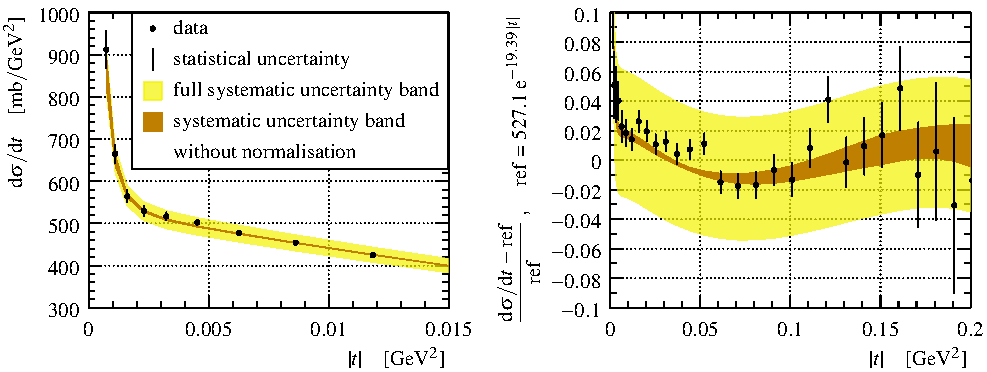
\includegraphics[width=18cm]{fig/t_dist_tabulation.pdf}
\vskip-3mm
\caption{%
Differential cross-section from Table \ref{tab:data} with statistical (bars) and systematic uncertainties (bands). The blue band represents all systematic uncertainties, the yellow one all but normalisation. LEFT: a low-$|t|$ zoom of the differential cross-section, with the rise due to the Coulomb interaction clearly visible. RIGHT: differential cross-section over the full $|t|$ range plotted relative to a reference exponential.
}
\label{fig:dsdt}
\end{center}
\end{figure*}


\begin{figure*}
\begin{center}
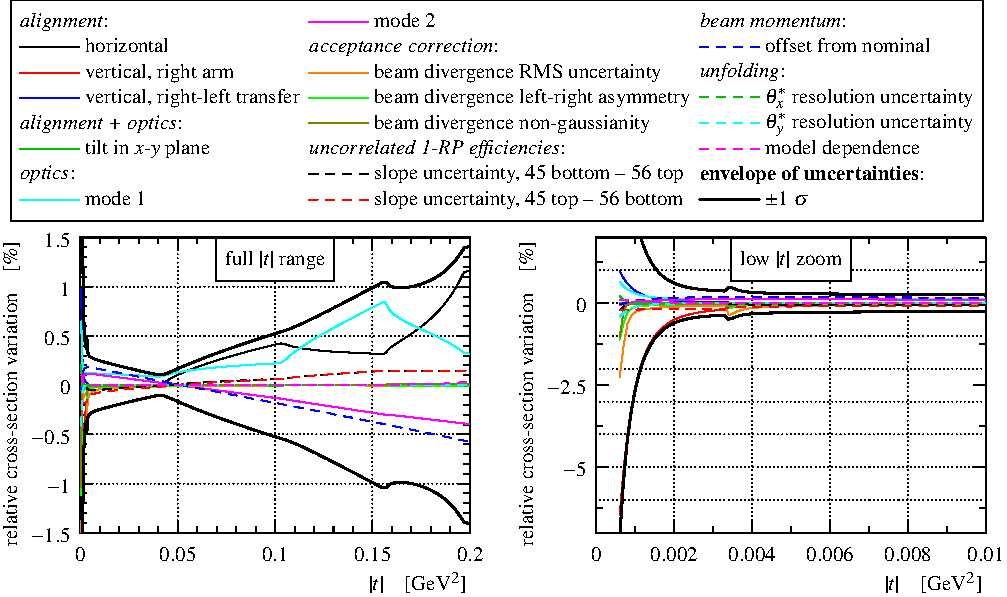
\includegraphics[width=18cm]{fig/systematic_uncertainties.pdf}
\caption{%
Impact of systematic uncertainties on the differential cross-section. 
LEFT: full $|t|$ range, RIGHT: low $|t|$ zoom.
The two contributions due to optics correspond to the two eigenvectors of the $\theta_x^*$, $\theta_y^*$ scaling covariance matrix (see section \ref{sec:optics}).
}
\label{fig:syst unc}
\end{center}
\end{figure*}
